% Created 2013-10-20 Sun 13:44
\documentclass[11pt]{article}
\usepackage[latin1]{inputenc}
\usepackage[T1]{fontenc}
\usepackage{fixltx2e}
\usepackage{graphicx}
\usepackage{longtable}
\usepackage{float}
\usepackage{wrapfig}
\usepackage{soul}
\usepackage{textcomp}
\usepackage{marvosym}
\usepackage{wasysym}
\usepackage{latexsym}
\usepackage{amssymb}
\usepackage{hyperref}
\tolerance=1000
\providecommand{\alert}[1]{\textbf{#1}}

\title{*Statistics and Data Analysis Notes}
\author{}
\date{\today}
\hypersetup{
  pdfkeywords={},
  pdfsubject={},
  pdfcreator={Emacs Org-mode version 7.9.3f}}

\begin{document}

\maketitle

\setcounter{tocdepth}{3}
\tableofcontents
\vspace*{1cm}
\begin{itemize}
\item Peng is researcher on air pollutation and health effects.
\end{itemize}

\section{Week One Lectures}
\label{sec-1}
\subsection{What Makes R Different?}
\label{sec-1-1}

\begin{itemize}
\item hybrid of command line and programming interface - best and worst
  of both worlds.
\end{itemize}
\subsection{How to get help}
\label{sec-1-2}

\begin{itemize}
\item People may not know you or what you mean
\item Use resources:
\end{itemize}
-- Search Forum
-- Search Web
-- Read the Manual
-- Read FAQ
-- Inpection and experimentation
-- Talk to a Friend
-- Read the source code

\begin{itemize}
\item Ask Questions
\end{itemize}
-- let people know you looked at above
-- reproducable example (test data)
-- expected output to be (maybe you are wrong) and what comes out
needs to be solved
-- version information and package information
-- Type of OS you are using

\begin{itemize}
\item Send email to forum
\end{itemize}
-- Subject lines should be useful
-- Describe big picture and goal
-- Specific problem (minimum amount of information)

\begin{itemize}
\item Do not:
\end{itemize}
-- Don't claim you found a bug
-- No groveling (lazy didn't do above)
-- No multiple mailing lists at once
-- Don't ask others to debug code
\subsection{Background and Overview}
\label{sec-1-3}
\subsubsection{History of R}
\label{sec-1-3-1}

\begin{itemize}
\item R is dialect of S
\item S developed at Bell Labs (1976)
\item Version 4 1998
\item R is implimentation of S
\item 1991 R created by Ross Ihaka and Robert Gentleman
\item Announced in 1993 to public
\item Martin Machler convinved Ross and Robert to release R under GNU GPL
\item 2000 R 1.0.0 released
\item 2012 R 2.15.1 released
\end{itemize}
\subsubsection{Features of R}
\label{sec-1-3-2}

\begin{itemize}
\item will run on almost any OS (including PlayStation 3)
\item functionality is divided into packages
\item strong graphics
\item GPL (4 freedoms)
\end{itemize}
\subsubsection{Drawbacks}
\label{sec-1-3-3}

\begin{itemize}
\item 40 year old technology is platform
\item little support for 3d graphics (but have improved)
\item no corporate help line or contact for feature (you have to build it)
\item objects stored in physical memory (some advancements made)
\item not ideal for all situations
\end{itemize}
\subsubsection{Design of system}
\label{sec-1-3-4}

\begin{itemize}
\item Base download
\end{itemize}
-- Base system (base, utils etc)
-- Recommend packages (boot, nlme etc.)

\begin{itemize}
\item 4,000 User contributed packages on CRAN (but must meet certain level
  of quality)
\item \href{http://bioconductor.org}{http://bioconductor.org} project (genomic and biological data
  analysis)
\item Others
\end{itemize}
\subsubsection{Documentation}
\label{sec-1-3-5}


\begin{itemize}
\item An introduction to R
\item Writing R extensions
\item R Data Import/Export
\item R installation and Admistration
\item R Internals
\end{itemize}
\subsection{Data Types}
\label{sec-1-4}

Everything in R is an object:
\subsubsection{five basic `atomic' classes of objects}
\label{sec-1-4-1}

\begin{itemize}
\item character
\item numeric
\item integer
\item complex numbers
\item logical
\end{itemize}
\subsubsection{vector}
\label{sec-1-4-2}

\begin{itemize}
\item contain only objects of same class
\item but a list can have different classes
\item empty vectors created with vector() function with args: class and length
\end{itemize}
\subsubsection{numbers}
\label{sec-1-4-3}

\begin{itemize}
\item generally as double precision
\item can explicitly define an integer with L after number
\item Inf is infinity can be plus or minus
\item NaN is undefined (not a number)
\end{itemize}
\subsubsection{Attributes}
\label{sec-1-4-4}

\begin{itemize}
\item can be part of an object in R:
\item names, dimnames
\item dimensions
\item class
\item length (length of vector etc.)
\item other user-defined attributed/metadata
\item General function attributes() can set or modify attributes
\end{itemize}
\subsubsection{Expressions}
\label{sec-1-4-5}


\begin{verbatim}
 <- assignment operator
# Error: needs things on both sides
print(x)
[1] "1"
> msg <- "hello"
# hash is comment character
\end{verbatim}
-Evaluation by R engine may or may not show anything.
-- assignment does not show anything
-- but putting a variable in the engine will autoprint
-- same as calling print function
-- with print the double square brackets shows what element of vector is being
shown

\begin{verbatim}
x <- 1:20 the : creates a sequence 1 to 20
\end{verbatim}
\begin{itemize}
\item c() concatnates objects to create vectors
\item vector can initialize vectors:
\end{itemize}

\begin{verbatim}
x <- vector("numeric", length=10) # initializes vector with 0's
\end{verbatim}
\begin{itemize}
\item concatnating will coerce classes:
\end{itemize}

\begin{verbatim}
y <- c(1.7, "a") ## character is least common denominator
\end{verbatim}
-- logical concatnated to numeric is coerced to numeric
-- logical and character coerced to character
-- coercsion will happen behind the scenes
-- you can coerce explicitly (as. character, as.numeric etc)
-- nonsensical coercion will result in NA's
\subsubsection{Matrices}
\label{sec-1-4-6}

\begin{itemize}
\item special type of vectors
\item has dimension attribute
\item created by matrix function
\item by default matrix is filled by columnwise (can be switched)
\item can create matrix by assigning dim attribute eg. dim(x) <= c(5,2)
\item column binding (cbind) and row binding (rbind) can create matrix
\end{itemize}
\subsubsection{List}
\label{sec-1-4-7}

\begin{itemize}
\item like vector but each object can be different
\item used to carry around data in functions
\end{itemize}
\subsubsection{Factors}
\label{sec-1-4-8}

\begin{itemize}
\item used to represent catagorical data
\item treated special by models
\item can be ordered (hierarchical) and unordered
\item factors are better than integers that represent things (self
  explaining)
\item levels is a special attribute of factors
\item unclass function strips out levels - create an integer with key as
  to what they mean
\item create an ordering using the levels= argument in the factor function
\end{itemize}
\subsubsection{missing values}
\label{sec-1-4-9}

\begin{itemize}
\item NA or NaN. NA is missing, NaN is not a number
\item NaN is also NA, but NA is not NaN.
\end{itemize}
\subsubsection{Data frame}
\label{sec-1-4-10}

\begin{itemize}
\item stores tabular data
\item special type of list, with each having the same length
\item columns can be different types
\item has attributes row.names
\end{itemize}
-data.matrix() can convert data.frame to matrix (with coercion)
\subsubsection{Names}
\label{sec-1-4-11}

\begin{itemize}
\item can assign names to elements (self describing data!)
\item matrix can have names (set with dimnames)
\end{itemize}
\subsection{Sub-setting Data}
\label{sec-1-5}
\subsubsection{vector operators}
\label{sec-1-5-1}

\begin{itemize}
\item single square bracket - always returns same type of object. Can be
  used to get more than one object
\end{itemize}

\begin{verbatim}
x[x>4], x[1:4], c[c=="fruit"] #etc
\end{verbatim}
-- NEAT can use lexical orders

\begin{verbatim}
x[x>"a"] # returns "b","c", "d", ...
\end{verbatim}
-- logical indexing

\begin{verbatim}
u <- x > "a" ; x [u]
\end{verbatim}
\begin{itemize}
\item double square bracket - list of data frame. Object returned may not be same class
  as parent object.
\item dollar sign - list or data frame that have name.
\end{itemize}
\subsubsection{matrix}
\label{sec-1-5-2}

\begin{itemize}
\item matrices can be subsetted with i,j notation. leave i or j to get
  row or columns.
\item subset single number or row of matrix you get a vector (not a 1 by 1
  matrix) turn off default with drop=FALSE
\end{itemize}
\subsubsection{list}
\label{sec-1-5-3}

\begin{itemize}
\item single square bracket -
\end{itemize}

\begin{verbatim}
x <- list(foo=1:4, bar=0.6)
x[1] #returns list can also use ["name"]
\end{verbatim}
\begin{itemize}
\item double bracket reutrns sequence 1,2,3,4
\item can not use double bracket for multiple objects
\item can use double bracket with computed index:
\end{itemize}


\begin{verbatim}
name <- "foo"
x[[[[name]]]]  #returns "x[[[["foo"]]]"
x[[[[c(1,3)]]]] #extracts 3rd item of 1st object
\end{verbatim}

\begin{itemize}
\item partial matching
\end{itemize}

\begin{verbatim}
x <- list(aardvark = 1:5) ; x$a matches x$aardvark but double
\end{verbatim}

bracket does not partial match unless exact=FALSE argument is made
\subsubsection{removing NA's}
\label{sec-1-5-4}


\begin{verbatim}
x[!is.na(x)] subsets non NA values
  good <- complete.cases(x,y) #gives non-missing across both vectors;
  x[good]; y[good]
  good <- complete.cases(airquality); airquality[good,][1:6]
\end{verbatim}
\subsection{Vecotorized Operations}
\label{sec-1-6}

\begin{itemize}
\item Feature in many languages - avoids looping
\item two vectors added together (x and y)
\end{itemize}
-- each element is added together when x and y are same length
\begin{itemize}
\item greater than less than operators return logical vector
\end{itemize}
-other arithemetic operations are vector operations
\begin{itemize}
\item Can work with matrix multiplication without the \% sign around it it
  is element wise operation
\item makes code easier to write
\end{itemize}
\subsection{Reading and writing data in R}
\label{sec-1-7}

\begin{itemize}
\item read.table, read.csv
\item readLines for reading lines of text file
\item source R code files
\item dget for reading R code files
\item load for reading saved workspaces
\item unserialize for reading single R objects in binary form
\end{itemize}
\subsubsection{write data}
\label{sec-1-7-1}

\begin{itemize}
\item write.table
\item writeLines
\item dump
\item dput
\item save
\item serialize
\end{itemize}
\subsubsection{more on read.table}
\label{sec-1-7-2}

\begin{itemize}
\item file: connection (string)
\item header: is first line a header
\item sep: how columns are separated
\item colClasses - a vector of column classes
\item nrows - number of rows in dataset
\item comment.char - character string indicating the comment character
\item skip = number of rows to skip
\item stringsAsFactors = should character variables be coded as a factor?
\item read.table has some intuitive defaults - telling up front makes R
  more efficient
\item read.csv is for csv files (defualt separator is command and
  header=TRUE)
\end{itemize}
\subsubsection{large data}
\label{sec-1-7-3}

\begin{itemize}
\item read help page
\item estimate memory size (if not enough RAM your done)
\item set comment = ``'' if no comment lines
\end{itemize}


\begin{verbatim}
initial <- read.table("datatable.txt", nrows=100)
classes <- sapply(initial, class)
tabAll <- read.table("datatable.txt", colClasses = classes)
\end{verbatim}

\begin{itemize}
\item Set nrows (if known) helps with memory usage - can overestimate
\end{itemize}
\subsubsection{R with large datasets}
\label{sec-1-7-4}

\begin{itemize}
\item how much memory does my computer have?
\item what other applications are in use?
\item multiuser system?
\item OS 32 or 64 bit?
\item rough calc of memory = 1.5 million by 120 columns all numeric:
\end{itemize}
-- 1.5 million x 120 x 8 bytes/numeric = 1.34 GB of physical memory
-- going to need a little more for overhead (twice as much needed for
read.table)


<s and TAB will create code block!
\subsubsection{dumping and dputting}
\label{sec-1-7-5}

\begin{itemize}
\item text format, but contain metadata (type of data in each
  object). Potentially recoverable.
\item read data source and dget.
\item Editable format. Can recover if corrupted. Longer lived.
\item Version control is workable with textual data (track changes)
\item Unix philosophy - store the data as text
\item BIG
\end{itemize}


\begin{verbatim}
y <- data.frame(a=1, b="a))
dput(y)

structure(list(a=1, b=structure(1L, .Label ="a",
class -"factor")), ..

dput(y, file="y.R)

# puts file y.R with y in it.

dump(c("x","y"), file="data.R")

source("data.R") # reconstructs objects
\end{verbatim}
\subsubsection{Connections}
\label{sec-1-7-6}

\begin{itemize}
\item \emph{file} opens a connection (to the file of course!)
\item \emph{gzfile} opens gzip file connection
\item \emph{bzfile} opens connection to compressed bzip2
\item \emph{url} opens a connection to a webpage
\end{itemize}

file arguments \emph{open} = `r' is read only; `w' is writing;
`a' is appending; `rb' `wb' `ab' is reading writing or appending
binary  mode (Windows).
\begin{itemize}

\item Gzip and file Connections\\
\label{sec-1-7-6-1}%
\begin{verbatim}
con <- file("foo.txt", "r")
data <- read.csv(con)
close(con)

# smae as

data <- read.csv(foo.txt")

con <- gzfile("words.gz")
x <- readLines(con,10)
x
close(con)
\end{verbatim}

\item HTML FILE Connections\\
\label{sec-1-7-6-2}%
\begin{verbatim}
con <- url("http//www.jhsph.edu", "r")
x <- readLines(con)
head(x)
close(con)
\end{verbatim}

\end{itemize} % ends low level
\subsubsection{Edit Code and Setting up Working Directory}
\label{sec-1-7-7}




\begin{verbatim}
getwd()
read.csv("mydata.csv") # can return error if file is not there.

setwd() # will change directory
\end{verbatim}

When you read or write data they will be sent to the working
directory. Peng suggests creating one directory.
\begin{itemize}

\item Editing script
\label{sec-1-7-7-1}%
\begin{itemize}
\item can use R's script editor
\item move between editor and R using Cntrl-A Cntrl -C Cntrl-V
  (select all - copy-paste)
\item save file in coursera folder you should create then use
\end{itemize}

\begin{verbatim}
source("mycode.R")
\end{verbatim}

assuming you've got the right directory. He did not go into hotkeys
(to send code to R) or any IDE's such as R Studio or Emacs (insert
boo's here)

\end{itemize} % ends low level
\subsubsection{Lecture on Macs (I will never afford one I suppose!)}
\label{sec-1-7-8}
\subsubsection{Structure of R Object}
\label{sec-1-7-9}


\begin{verbatim}
str()
\end{verbatim}

Is the most important function in R according to Peng. Diagnostic
function and an alternative to summary.

\begin{itemize}
\item useful for large lists
\item 1 line of output per object
\end{itemize}


\begin{verbatim}
str(str)
#function (object, ...)

str(lm) # etc.

x <- rnorm(100,2,4)
summary(x) # five num summary
str(x) # gives class, 100 elements, first 5 numbers

f <- gl(40,10)

str(f) # returns information of factor levels and first couple
of numbers.

summary(f) # counts on each levels

data(airquality)
head(airquality)
str(airquality) # tells us its a data.frame, first observations on
each of the vectors (and their classes).

m <- matrix(rnorm(100),10,10)
str(m) will tell us its a matrix (10 by 10) and first couple of obs.

s <- split(airquality, airquality$Month)

str(s) # givens the list of data frames each data.frame str() applied
to it. (nice!)
\end{verbatim}

Yep its definitely useful!
\section{Week Two Lectures}
\label{sec-2}
\subsection{Control Structures}
\label{sec-2-1}

typically used in functions
\begin{itemize}
\item if, else
\item for
\item while
\item repeat
\item break
\item next
\item return
\end{itemize}
\subsubsection{if, else and if else}
\label{sec-2-1-1}


\begin{verbatim}
rm(list=ls())
x <- 2
if ( x > 3 ){
    y <- 3
} else {
    y <- 0
}
print(y)

# or can value to assign to y
x <- 10
y <- if ( x >3 ){
    10
} else {
    0
}
print(y)

# if else
x <-3
y <- if (x<3){
10
} else if (x>3){
11
} else {
12
}
print(y)
\end{verbatim}

\begin{verbatim}
 [1] 0
 [1] 10
 [1] 12
\end{verbatim}
\subsubsection{for loops}
\label{sec-2-1-2}



\begin{verbatim}


for ( i in 1:10){
    print(i)
}
\end{verbatim}


\begin{verbatim}
[1] 1
[1] 2
[1] 3
[1] 4
[1] 5
[1] 6
[1] 7
[1] 8
[1] 9
[1] 10
\end{verbatim}

Loop index i, cycles through. Don't overwright.

Different ways of using for loop (all do the same thing):


\begin{verbatim}
x <- c("a", "b","c","d")

for(i in 1:4){
print(x[i])
}

for (i in seq_along(x)) {
print(x[i])
}
# don't need numbers can use letters
for(letter in x){
print(letter)
}

for (i in 1:4) print(x[i]) # single expression, compact style

# Nested

x <- matrix(1:6,2,3)
for(i in seq_len(nrow(x))){

for(j in seq_len(ncol(x))){
print(x[i,j])
}
}
\end{verbatim}


\begin{verbatim}
[1] "a"
[1] "b"
[1] "c"
[1] "d"
[1] "a"
[1] "b"
[1] "c"
[1] "d"
[1] "a"
[1] "b"
[1] "c"
[1] "d"
[1] "a"
[1] "b"
[1] "c"
[1] "d"
[1] 1
[1] 3
[1] 5
[1] 2
[1] 4
[1] 6
\end{verbatim}

Nested loops beyond 2 levels is difficult to comprehend can ususally
use functions to get by without.
\subsubsection{While}
\label{sec-2-1-3}

Other looping. Takes a logical expression - while TRUE will run loop.


\begin{verbatim}
count <- 0
while(count<10){
print(count)
count <- count +1
}

#Random Walk
walk <- NULL
z <- 5
while(z >=0 && z <=100000){
walk <- c(walk, z)
coin <- rbinom(1,1,0.5)
if(coin==1) { ## random walk
    z <- z +1
} else {
    z <- z -1
}
}

plot(walk, type="l", main="A Random Walk starting at 5, stops at 0 or a million")
\end{verbatim}

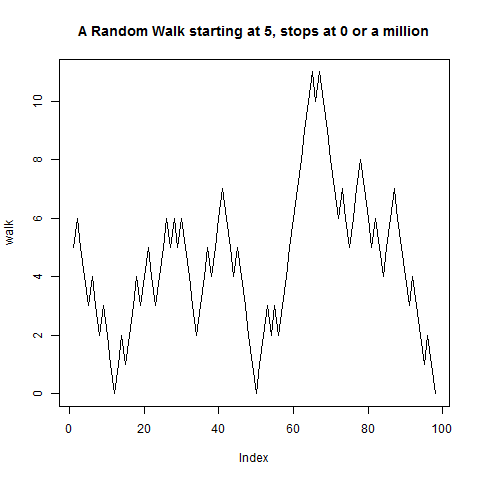
\includegraphics[width=.9\linewidth]{walk1.png}

\begin{itemize}
\item Can produce an infinite loop
\item Conditions evaluated from left to right
\item \&\& single logical value is used
\end{itemize}
\subsubsection{repeat loops}
\label{sec-2-1-4}

\begin{itemize}
\item need to call break or it runs forever
\end{itemize}

\begin{verbatim}
x0 <-1
tol <- 1e-8

repeat{
x1 <- computeEstimate()

if(abs(x1-x0) < tol){
    break
}else{
    x0 <-x1
}
}
\end{verbatim}
\begin{itemize}
\item Uses tolerance to keep looking at algorythm until tolerance value
  is met. BUT sometimes will not converge - so we should have a max
  iterations argument - use a for loop and it will eventually reached
  limit and stop.
\end{itemize}
\subsubsection{next}
\label{sec-2-1-5}

\begin{itemize}
\item used to skip a certain part of loop:
\end{itemize}

\begin{verbatim}
for(i in 1:25){
if (i<=20){
        ## skip the first 20 iterations
        next
}
print(i)
}
\end{verbatim}

\begin{verbatim}
 [1] 21
 [1] 22
 [1] 23
 [1] 24
 [1] 25
\end{verbatim}
\subsubsection{return}
\label{sec-2-1-6}

\begin{itemize}
\item Exit entire function and return a value that you pass it.
\item Interupts everything
\end{itemize}
\subsubsection{Final Notes}
\label{sec-2-1-7}

\begin{itemize}
\item Infinite loops should be looked out for
\item Looping functions are generally used with apply (especially when
  ineracting with data).
\end{itemize}
\subsection{Control Structures}
\label{sec-2-2}

\begin{itemize}
\item Transition from User to Programmer.
\end{itemize}
\subsubsection{Basics of writing functions}
\label{sec-2-2-1}

\begin{itemize}
\item created using functions directive
\item R functions are class ``function'':
\end{itemize}

\begin{verbatim}
f <- function(<args>){

## DO anything
}
\end{verbatim}

\begin{itemize}
\item Functions are first class functions. They can be treated like
  any other objects
\item can be passed to other functions
\item nested so you can define a function inside another function
\item the return value of the function = last expression in the body to
  be evaluated
\item Functions have \emph{names arguments} which can have \emph{default values}
\item \emph{Formal arguments} are arguments that are included in the function
  definition
\item The \emph{formals} function: returns list of (formal) arguments of a
  function (included inside the ())
\item Not all functions have formal arguments ?
\item Functions can have missing arguments or might have defaults
\item R function arguments can be matched by position or name:
\end{itemize}

\begin{verbatim}
mydata <- rnorm(1000)
formals(sd)

sd(mydata)
sd(mydata, na.rm=FALSE)

# OR
sd(mydata, FALSE)

# or
sd(x=mydata, na.rm=FALSE)

# or

sd(na.rm=FALSE, mydata)

# first argument is matched to mydata (after assigning mydata)
# Reversing arguments is a bad idea

#equivalent:
lm(data=mydata, y~x, model=FALSE, 1:100)
lm(y ~x, mydata, 1:100,  model=FALSE)
\end{verbatim}

\begin{itemize}
\item names arguments are used on the command line (order not so important)
\item functions can be partially matched (if it has a long name) looks for unique match. The order of preference is:
\item check for exact match
\item partial match
\item positional match
\end{itemize}
\subsubsection{LAZY EVALUATION}
\label{sec-2-2-2}

\begin{itemize}
\item Arguments are evaluated only as needed.
\end{itemize}

\begin{verbatim}

f <- function(a,b){
     a^2
}
f(2)
\end{verbatim}

\begin{verbatim}
 [1] 4
\end{verbatim}

\begin{itemize}
\item This function never actually uses the argument b, so called f(2)
  will NOT produce an error because a=2 (and it does not care about b).
\item BUT:
\end{itemize}


\begin{verbatim}
f <- function(a,b){
print(a)
print(b)
}

f(45)
\end{verbatim}

\begin{verbatim}
 [1] 45
 Error in print(b) (from #3) : argument "b" is missing, with no default
\end{verbatim}

\begin{itemize}
\item Produces this:
\end{itemize}

\begin{itemize}
\item up to print(a) we are ok, but the print(b) throws the error (LAZY
  EVALUATION) - executes until it bonks on an error.
\end{itemize}
\subsubsection{``\ldots{}'' argument.}
\label{sec-2-2-3}

\begin{itemize}
\item Often used to extend a function.
\item so if you were calling another function inside your function, you
  can use \ldots{} to pass the arguments to the extended function
\item Generic functions (we will talk about this later).
\item dispatch methods for different types of data
\item \ldots{} is handy if known number of arguments can not be known.
\item paste is example.
\end{itemize}

\begin{verbatim}
args(paste)
args(cat)
\end{verbatim}

\begin{verbatim}
 function (..., sep = " ", collapse = NULL) 
 NULL
 function (..., file = "", sep = " ", fill = FALSE, labels = NULL, 
     append = FALSE) 
 NULL
\end{verbatim}

\begin{itemize}
\item One catch is that anything after \ldots{} must be \underline{EXPLICIT and $_{\mathrm{CANNOT}}$ be  $_{\mathrm{PARTIALLY}}$ MATCHED}
\end{itemize}
\subsubsection{A Diversion on Binding Values to a Symbol}
\label{sec-2-2-4}



\begin{verbatim}
lm <- function(x) {x *x}
lm
\end{verbatim}

\begin{itemize}
\item how does R know what you are talking about?
\item \emph{lm} in \emph{stats package}
\item \emph{lm} in you just defined.
\item R binds a value to a symbol.
\item Searches through series of \emph{Environments} for a match.
\item Search .GlobalEnv environment first (users workspace)
\item Then search namespaces of search list (all R packages loaded in R)
\item \emph{Base} package is last
\end{itemize}


\begin{verbatim}
search()
\end{verbatim}

\begin{verbatim}
 function(x) {x *x}
  
 [1] ".GlobalEnv"        "package:stats"     "package:graphics" 
  [4] "package:grDevices" "ESSR"              "package:utils"    
  [7] "package:datasets"  "package:methods"   "Autoloads"        
 [10] "package:base"
\end{verbatim}

\begin{itemize}
\item list of packages are dynamic depending on session - library
  installs namespace right behind global environment.
\end{itemize}


\begin{verbatim}
library(NADA)
search()
\end{verbatim}


\begin{verbatim}
Loading required package: survival
Loading required package: splines

Attaching package: 'NADA'

The following object is masked from 'package:stats':

    cor
 [1] ".GlobalEnv"        "package:NADA"      "package:survival" 
 [4] "package:splines"   "package:stats"     "package:graphics" 
 [7] "package:grDevices" "ESSR"              "package:utils"    
[10] "package:datasets"  "package:methods"   "Autoloads"        
[13] "package:base"
\end{verbatim}

\begin{itemize}
\item you can have a vector names `c' (and it would not interfere
  normally with function `c') (separate namespaces for functions and non-functions)
\end{itemize}
\subsubsection{Scoping Rules (Lexical Scoping)}
\label{sec-2-2-5}

\begin{itemize}
\item makes it different from S
\item Scoping rules determine how value is bound to variable.
\item Useful for simplifying calculations
\item Sometimes called \emph{static scoping} and alternative called \emph{dynamic   scoping}
\item R uses search list to bind a value to a symbol
\item Consider this:
\end{itemize}

\begin{verbatim}
f <- function(x,y){
x^2 + y / z
}
\end{verbatim}


This function has 2 formal args, x and y. There is a symbol z in the
body. z is a free variable\ldots{} how assign value to z is the scoping
rules.

\begin{itemize}
\item lexical scoping looks for value in the environment in which the
  function was defined.
\item x <- 3.14
\item y <- data.frame(x=rnorm(100), y=rnorm(100))
\item and environment is a symbol-value pair
\item every environment has a parent environment
\item create a function and assign to an environment it creates a closure
\item if a free variable is encountered, R looks in environment the
  function was defined in. If not. Search then looks in the parent
  environment until it hits the top-level environment. If can't find
  anything it throws an error
\item Possible to define a function outside .GlobalEnv
\end{itemize}
-WHY DOES THIS MATTER?
\begin{itemize}
\item DEFINE GLOBAL VARIABLES
\item DEFINE FUNCTIONS INSIDE OTHER FUNCTIONS
\item EXAMPLE constructor functions that construct other functions
\end{itemize}
make power returns a function (one function can make many functions)

\begin{verbatim}
make.power <- function(n){
pow <- function(x){
x^n
}
pow
}

cube <- make.power(3)
square <- make.power(2)

cube(3)
square(3)
\end{verbatim}

\begin{verbatim}
 [1] 27
 [1] 9
\end{verbatim}

-Produce some different results

\begin{itemize}
\item how do you know what is in the functions environment>
\end{itemize}

\begin{verbatim}
ls(environment(cube))
ls(environment(square))

get("n", environment(cube))
get("n", environment(square))
\end{verbatim}

\begin{verbatim}
 [1] "n"   "pow"
 [1] "n"   "pow"
 [1] 3
 [1] 2
\end{verbatim}

\begin{itemize}
\item how the new function knows what to do (each has its own environment
  with things definitions
\item \emph{dynamic scoping} would do this - a free variable looks up value in
  environment where the function was defined.
\item When a function is defined in the .GlobalEnv it will appear to be
  \emph{dynamic scoping}
\end{itemize}


\begin{verbatim}
rm(list=ls())
g <- function(x){
a <- 3
x + a + y
}

g(2)
y<-3
g(2)
\end{verbatim}

\begin{verbatim}
 Error in g(2) (from #3) : object 'y' not found
 [1] 8
\end{verbatim}

\begin{itemize}
\item Other languages with \emph{lexical scoping}
\item Scheme
\item Perl
\item Python
\item Common Lisp (\emph{theorem: all languages converge to Lisp})
\end{itemize}
\begin{itemize}

\item Consequence of Lexical Scoping
\label{sec-2-2-5-1}%
\begin{itemize}
\item ALL OBJECTS GET STORED IN PHYSICAL MEMORY!
\item Limits big data
\item Every function has to have a pointer to its defining environment
\item in S+ free variable looked up in .GlobalEnv
\end{itemize}

\end{itemize} % ends low level
\subsection{Optimization}
\label{sec-2-3}

\begin{itemize}
\item optim and nl, and optimize require pass a function to them, whose
  argument is a vector of parameters
\item finds minimum or maximize (usually log-likelihood)
\item lexical scoping makes it easy
\item create constructor function that constructs the objective function
\item have data etc. in environment (like baggage)
\item example:
\end{itemize}

\begin{verbatim}
rm(list=ls())
make.NegLogLik <- function(data, fixed=c(FALSE,FALSE)){
    params <- fixed
    function(p){
        params[!fixed] <- p
        mu <- params[1]
        sigma <- params[2]
        a <- -0.5 * length(data) * log(2*pi*sigma^2)
        b <- -0.5 * sum((data -mu)^2)/(sigma^2)
        -(a+b)
        }
}
\end{verbatim}


\begin{itemize}
\item Note Optimization functions in R \emph{minimize} functions, so you need
  to use the negative log-likelihood
\item fit normal distribution.
\end{itemize}


\begin{verbatim}

set.seed(1); normals <- rnorm(100,1,2)
nLL <- make.NegLogLik(normals)
nLL
ls(environment(nLL))
\end{verbatim}


\begin{verbatim}
function(p){
        params[!fixed] <- p
        mu <- params[1]
        sigma <- params[2]
        a <- -0.5 * length(data) * log(2*pi*sigma^2)
        b <- -0.5 * sum((data -mu)^2)/(sigma^2)
        -(a+b)
        }
<environment: 0x04add384>
[1] "data"   "fixed"  "params"
\end{verbatim}

\begin{itemize}
\item environment is some fancy hex. number e.g. 0x165b1a4
\item data variable is a free variable. But data can look up in the
  parent environment.
\item now can call optim.
\end{itemize}


\begin{verbatim}
optim(c(mu=0, sigma=1), nLL)$par

print("fix sigma = 2")
nLL <- make.NegLogLik(normals, c(FALSE, 2))
optimize(nLL, c(-1,3))$minimum

print("fix mu =1")
nLL <- make.NegLogLik(normals, c(1, FALSE))
optimize(nLL, c(1e6,10))$minimum
\end{verbatim}

\begin{verbatim}
       mu    sigma 
 1.218239 1.787343
 [1] "fix sigma = 2"
 [1] 1.217775
 [1] "fix mu =1"
 [1] 10.00005
\end{verbatim}


\begin{itemize}
\item plotting a log-liklihood
\end{itemize}

\begin{verbatim}
nLL <- make.NegLogLik(normals, c(1, FALSE))
x <- seq(1.7, 1.9, len=100)
y <- sapply(x,nLL)
plot(x, exp(-(y-min(y))), type="l")
\end{verbatim}

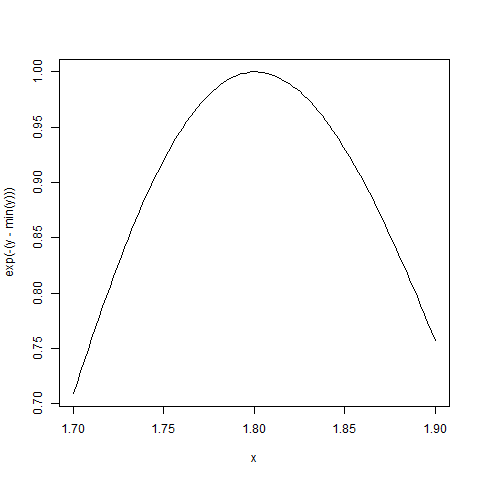
\includegraphics[width=.9\linewidth]{LL2.png}


\begin{verbatim}
nLL <- make.NegLogLik(normals, c(FALSE, 2))
x <- seq(0.5, 1.5, len=100)
y <- sapply(x,nLL)
plot(x, exp(-(y-min(y))), type="l")
\end{verbatim}

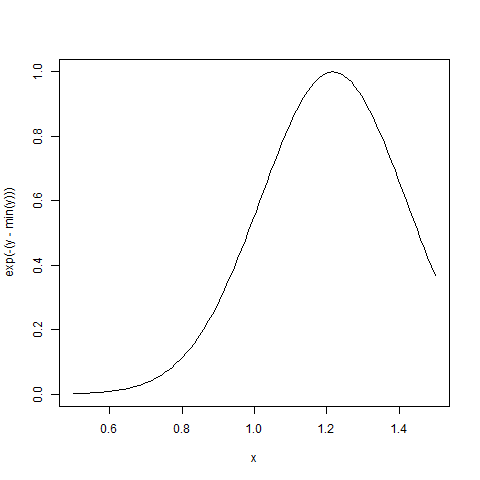
\includegraphics[width=.9\linewidth]{LL3.png}


\begin{verbatim}
x <- rlorm(1099)
summary(x)
function(x){
    rnorm(n=x)
}
\end{verbatim}
\subsection{loops lapply}
\label{sec-2-4}


\begin{itemize}
\item lapply - loop over a list and evaluation a function for each
  element in the list
\item sapply - same as sapply but try and simplify result (Hadly was not
  a found fan of this)
\item apply - apply function over margins of array
\item tapply - apply function over subset of vector
\item mapply- multivariate version of lapply
\item split is an aux. function and is useful in conjunction with lapply
  (splits into a list of sub-pieces)
\end{itemize}
\subsubsection{lapply}
\label{sec-2-4-1}

\begin{itemize}
\item takes 3 arguments
\item X (a list). If X is not a list it will be coerced into a list
\item FUN ( a function)
\item \ldots{} (extra arguments)
\item actual looping is done in C
\end{itemize}


\begin{verbatim}
  x <- list(a=1:5, b=rnorm(10))
  lapply(x, mean)

x <- list(a=1:4, b=rnorm(10), c=rnorm(20,1), d= rnorm(100,5))
lapply(x,mean)

x <- 1:4

lapply(x,runif)

#suppose wanted nondefault behavior

lapply(x, runif, min=0, max=10) # using the ... part of lapply
\end{verbatim}


\begin{verbatim}
$a
[1] 3

$b
[1] 0.3474802
$a
[1] 2.5

$b
[1] -0.1198232

$c
[1] 0.782726

$d
[1] 4.964196
[[1]]
[1] 0.7603133

[[2]]
[1] 0.1554012 0.8494571

[[3]]
[1] 0.9468178 0.5884192 0.5022508

[[4]]
[1] 0.189779918 0.001836858 0.877578062 0.134111338
[[1]]
[1] 0.2274122

[[2]]
[1] 9.391367 2.929487

[[3]]
[1] 1.643266 3.991026 4.595754

[[4]]
[1] 4.3403085 5.1700983 8.4624575 0.5516429
\end{verbatim}

\begin{itemize}
\item what goes in is coerced to a list and what comes out \emph{always} is a
  list.
\end{itemize}


\begin{verbatim}
x <- list(a=matrix(1:4, 2,2), b= matrix(1:6, 3,2))
x
# extract first column from matrix (need to create function to do this):
lapply(x, function(elt) elt[,1])

# function is gone at the end of lapply (an anonymous functions)
\end{verbatim}


\begin{verbatim}
$a
     [,1] [,2]
[1,]    1    3
[2,]    2    4

$b
     [,1] [,2]
[1,]    1    4
[2,]    2    5
[3,]    3    6
$a
[1] 1 2

$b
[1] 1 2 3
\end{verbatim}
\subsubsection{sapply}
\label{sec-2-4-2}

\begin{itemize}
\item will try and simplyfy results
\item for instance, if all elements in list that comes back has same
  length - it will create  vector (length 1) or matrix ( if greater
  than 1).
\item if can't it will return a list
\end{itemize}


\begin{verbatim}
x <- list(a=1:4, b=rnorm(10), c=rnorm(20,1), d= rnorm(100,5))
sapply(x,mean)
# returns vector
class(sapply(x,mean))

# error:

mean(x) # mean can not be directly applied to lists

What will this produce?
x <- list(rnorm(100), runif(100), rpois(100, 1))
sapply(x, quantile, probs = c(0.25, 0.75))
\end{verbatim}


\begin{verbatim}
         a          b          c          d 
2.50000000 0.01869495 1.07583942 5.06185108
[1] "numeric"
[1] NA
Warning message:
In mean.default(x) : argument is not numeric or logical: returning NA
Error: unexpected symbol in "What will"
          [,1]      [,2] [,3]
25% -0.7070224 0.2235743 0.00
75%  0.6800490 0.6987254 1.25
\end{verbatim}
\subsubsection{apply function}
\label{sec-2-4-3}

\begin{itemize}
\item it is common to apply to rows or columns of a matrix
\item apply is not really faster (but used to be true).
\item BUT it involves less typing. Good programers are always lazy.
\item X is an array
\item MARGIN is an integer that indicated what should be `retained'
\item \ldots{}
\end{itemize}


\begin{verbatim}
print("apply mean to margin 2")
x <- matrix(rnorm(200),20,10)
apply(x,2,mean)

print("apply to sum on margin 1")
apply(x,1,sum)
\end{verbatim}

\begin{verbatim}
 [1] "apply mean to margin 2"
  [1]  0.041597801 -0.007965326 -0.067736108 -0.442325546 -0.319348298
  [6] -0.160523432  0.054901735  0.037705261 -0.157675375  0.164261296
 [1] "apply to sum on margin 1"
  [1]  -5.4715707  -0.2029979   5.6390271   2.9712664  -4.7227922  -4.6296715
  [7]  -3.4401373   0.7085447   7.1666165   3.7750684  -2.2374511  -0.3080558
 [13]  -2.0090229  -6.1822947  -0.9802599 -10.4664555  -0.1741214   1.2001970
 [19]   1.2206894   1.0012615
\end{verbatim}

\begin{itemize}
\item column in margin 2 (the row dimension has been eliminated)
\item row is margin 1 (collapse the columns and preserve the rows)
\end{itemize}
\subsubsection{simple shortcuts}
\label{sec-2-4-4}

Quicker than apply (use these where you can)
\begin{itemize}
\item rowSums
\item rowMeans
\item colSums
\item colMeans
\end{itemize}
\begin{itemize}

\item apply in applying a function\\
\label{sec-2-4-4-1}%
\begin{verbatim}
x <- matrix(rnorm(200),20,10)
apply(x,1,quantile, probs=c(0.25,0.75))
\end{verbatim}


\begin{verbatim}
          [,1]       [,2]       [,3]       [,4]       [,5]       [,6]
25% -0.9042243 0.03361393 -0.6115209 -0.2969511 -0.5633196 -1.0058142
75%  0.5425005 0.98014390  0.7370544  0.2220907  0.5935485  0.6515029
          [,7]       [,8]       [,9]      [,10]     [,11]        [,12]
25% -0.8218577 -0.1700024 -0.7734633 -0.6774506 0.1271081 -0.001441062
75%  0.8648419  1.4822250  0.7245645  0.3245205 0.7244844  0.906033317
         [,13]        [,14]      [,15]      [,16]      [,17]      [,18]
25% -0.8746104 -1.954728372 -0.3022716 -0.8702418 -0.1525945 -1.1571882
75%  0.6324104  0.004634306  0.5467537  0.9206052  0.6926430  0.6431997
          [,19]      [,20]
25% -1.50837818 -0.8324263
75% -0.06477856  0.3844889
\end{verbatim}


\item Average of matrix in an array\\
\label{sec-2-4-4-2}%
\begin{verbatim}
a <- array(rnorm(2 * 2 * 10), c(2, 2, 10))
apply(a,c(1,2), mean)

print("rowMeans")
rowMeans(a, dims=2)
\end{verbatim}

\begin{verbatim}
             [,1]       [,2]
 [1,] -0.09143177 -0.4493842
 [2,] -0.08272792 -0.1027398
 [1] "rowMeans"
             [,1]       [,2]
 [1,] -0.09143177 -0.4493842
 [2,] -0.08272792 -0.1027398
\end{verbatim}

\begin{itemize}
\item average of a bunch of 2 by 2 matrices (collapsing 3rd dimension)
\item rowMeans can work as well (using dims=2).
\end{itemize}


\begin{verbatim}
x <- matrix(rnorm(200), 50, 4)
apply(x,1,sum)
apply(x,3,mean)
apply(x,2,min)
apply(x, c(1,2), mean)
\end{verbatim}


\begin{verbatim}
 [1]  0.05391193 -0.98725795  0.43950476  1.98447766  4.24731610 -2.22369827
 [7] -3.15906582 -2.72183522 -2.40786140 -0.17309768  3.96631043 -1.51406148
[13] -1.57396399 -1.98776564  1.85180050  3.09105187  0.24316866 -0.22275780
[19]  5.76285976 -1.30485739  4.06905865  0.95759103 -3.64273739  1.49945830
[25]  0.78987460 -2.00602076  1.55099746  0.37871842 -1.10517239 -0.67178684
[31] -3.14734641  0.87092184 -0.60548329 -1.11226137  1.44527850 -0.16108587
[37]  0.13958292 -2.05200753  2.35397435  0.95810458 -4.54757894  4.24600726
[43]  1.76835899 -0.75520723 -4.76132526 -1.49331871  0.98204482 -2.99763275
[49] -1.35146542 -1.62787599
Error in if (d2 == 0L) { : missing value where TRUE/FALSE needed
[1] -2.321491 -2.090846 -3.213189 -2.106118
              [,1]         [,2]        [,3]        [,4]
 [1,] -0.326489593  0.855519222 -0.09953695 -0.37558075
 [2,]  0.774005212 -0.819963127 -0.43985764 -0.50144240
 [3,]  0.785006401 -0.123602760 -0.71851145  0.49661258
 [4,]  0.763246080  0.254948236 -0.55459760  1.52088094
 [5,]  0.294808760  1.718926338  1.24548918  0.98809183
 [6,] -1.252355924 -0.958543528 -1.25892135  1.24612253
 [7,] -1.009503753 -1.604310262 -0.21538448 -0.32986733
 [8,]  0.751391195 -1.845609422 -2.47196171  0.84434471
 [9,] -1.308353513  0.555737185 -0.67416932 -0.98107576
[10,]  0.527540097 -0.060119191 -0.50129719 -0.13922141
[11,] -0.533539574  0.772086304  1.54232579  2.18543791
[12,] -0.398376014 -0.140839387 -0.96201807 -0.01282801
[13,] -0.789569450  0.393093926 -0.87217954 -0.30530893
[14,] -0.230141136  0.224218574 -1.39762962 -0.58421346
[15,]  0.877184842  0.023541985  0.17980517  0.77126850
[16,]  0.453733178 -0.622962660  1.15409199  2.10618936
[17,] -0.232464148  1.262009381 -1.19853361  0.41215704
[18,]  0.870005525 -0.405774043 -0.42572440 -0.26126488
[19,]  1.656003734  0.666763771  1.36630861  2.07378365
[20,] -0.006368929  0.164639155 -0.68429739 -0.77883022
[21,]  0.470489453  1.781524475  0.68551221  1.13153251
[22,]  0.278218649  0.711213964  0.38950354 -0.42134513
[23,] -0.977902941 -0.337691156 -1.30539592 -1.02174737
[24,] -0.926586142 -0.009148952  1.21688801  1.21830538
[25,]  1.919770463 -0.125309208  0.79517402 -1.79976067
[26,]  0.881277788 -2.090846097 -0.48820251 -0.30824994
[27,]  0.742081772  1.697393895 -0.90399345  0.01551524
[28,]  0.147573404  1.063881154 -0.39041842 -0.44231772
[29,]  0.485388565 -0.766616636  0.81406342 -1.63800773
[30,]  0.151856040  0.382007559 -0.56424928 -0.64140116
[31,]  0.041998754  0.241895904 -1.87420532 -1.55703574
[32,]  0.223422312 -1.132759411 -0.14290471  1.92316365
[33,] -1.010465086  1.489907414  0.77190401 -1.85682963
[34,]  2.401222102 -0.248247105 -1.15911793 -2.10611844
[35,]  0.801961790  0.183583708 -0.23791553  0.69764853
[36,] -0.251207959  0.404871009 -1.22219333  0.90744441
[37,]  1.212889371 -0.994124469  0.11680621 -0.19598820
[38,] -0.627258086 -1.085429330 -0.13249963 -0.20682049
[39,]  1.711158507 -0.048542555 -0.03368478  0.72504317
[40,] -0.394373553  0.576085601 -0.62232642  1.39871896
[41,] -2.321490856  0.073830532 -0.70936346 -1.59055515
[42,]  1.364119195  0.705945571  0.87144541  1.30449708
[43,]  1.132229133  0.334980103  0.10513802  0.19601173
[44,] -0.774316319  0.545387806 -0.18693527 -0.33934345
[45,] -1.410374966 -1.402905906 -3.21318853  1.26514414
[46,] -1.834527581  0.677053891 -1.27561870  0.93977369
[47,] -0.269013538 -0.789800446  0.76290632  1.27795249
[48,] -1.833928577 -0.465728889 -0.40681514 -0.29116014
[49,] -0.814468019 -0.104852065 -1.20831778  0.77617245
[50,]  0.163572122 -1.647851087 -0.43932266  0.29572563
\end{verbatim}

\end{itemize} % ends low level
\subsubsection{tapply}
\label{sec-2-4-5}

\begin{itemize}
\item function over a vector (pieces need  summary statistic over)
\item X is a vector
\item INDEX is a factor or list of factors (coerced into factors)
\item FUN is the function to be applied
\item \ldots{} contains other arguments to be passed to FUN
\item simplify (TRUE) like sapply simplification
\end{itemize}
 

\begin{verbatim}
x <- c(rnorm(10), runif(10), rnorm(10,1))
f <- gl(3,10) # generate levels
f
tapply(x,f,mean)
\end{verbatim}

\begin{verbatim}
  [1] 1 1 1 1 1 1 1 1 1 1 2 2 2 2 2 2 2 2 2 2 3 3 3 3 3 3 3 3 3 3
 Levels: 1 2 3
         1         2         3 
 0.4040684 0.4625386 0.8182498
\end{verbatim}

\begin{itemize}
\item if you don't simplify the results you will get back a list.
\end{itemize}

Can get a complicated thing back with this as well:

\begin{verbatim}

tapply(x,f,range)
\end{verbatim}

\begin{verbatim}
 $`1`
 [1] -0.7057714  2.6064445
 
 $`2`
 [1] 0.1394657 0.9299194
 
 $`3`
 [1] -0.6521103  3.3905767
\end{verbatim}
\subsubsection{split}
\label{sec-2-4-6}

\begin{itemize}
\item takes a vector or other objects and splits them by a factor or list
  of factors.
\item x is a vector
\item f is a factor or list of factors
\item drop indicated if empty factors will be dropped.
\end{itemize}


\begin{verbatim}
x <- c(rnorm(10), runif(10), rnorm(10,1))
f <- gl(3,10)
split(x,f)

# returns a list of length 3 with the 3 distributions in each
\end{verbatim}


\begin{verbatim}
$`1`
 [1] -0.36513161  1.38145425 -0.15331726 -0.25557163 -1.28862710  0.06526642
 [7]  1.03532642  2.26021579  1.31469628 -0.87002335

$`2`
 [1] 0.30743642 0.52829125 0.72822568 0.95355653 0.49599413 0.13201725
 [7] 0.60846876 0.99186858 0.09470967 0.89528346

$`3`
 [1] 0.57347013 0.07359575 0.07144208 0.28109940 0.58520943 0.99433211
 [7] 1.63344892 0.49081923 0.14299138 2.61616758
\end{verbatim}

\begin{itemize}
\item can also do some real fun here with plots:
\end{itemize}


\begin{verbatim}

lapply(split(x,f), mean)

lapply(split(x,f), hist)

print("Some more things to do")
library(datasets)
head(airquality)

# calculate mean for each month of all the columns

s <- split(airquality, airquality$Month)
lapply(s, function(x) colMeans(x[c("Ozone", "Solar.R", "Wind")], na.rm=TRUE))
\end{verbatim}


\begin{verbatim}
$`1`
[1] 0.3124288

$`2`
[1] 0.5735852

$`3`
[1] 0.7462576
$`1`
$breaks
[1] -2 -1  0  1  2  3

$counts
[1] 1 4 1 3 1

$density
[1] 0.1 0.4 0.1 0.3 0.1

$mids
[1] -1.5 -0.5  0.5  1.5  2.5

$xname
[1] "X[[1L]]"

$equidist
[1] TRUE

attr(,"class")
[1] "histogram"

$`2`
$breaks
[1] 0.0 0.2 0.4 0.6 0.8 1.0

$counts
[1] 2 1 2 2 3

$density
[1] 1.0 0.5 1.0 1.0 1.5

$mids
[1] 0.1 0.3 0.5 0.7 0.9

$xname
[1] "X[[2L]]"

$equidist
[1] TRUE

attr(,"class")
[1] "histogram"

$`3`
$breaks
[1] 0.0 0.5 1.0 1.5 2.0 2.5 3.0

$counts
[1] 5 3 0 1 0 1

$density
[1] 1.0 0.6 0.0 0.2 0.0 0.2

$mids
[1] 0.25 0.75 1.25 1.75 2.25 2.75

$xname
[1] "X[[3L]]"

$equidist
[1] TRUE

attr(,"class")
[1] "histogram"
[1] "Some more things to do"
  Ozone Solar.R Wind Temp Month Day
1    41     190  7.4   67     5   1
2    36     118  8.0   72     5   2
3    12     149 12.6   74     5   3
4    18     313 11.5   62     5   4
5    NA      NA 14.3   56     5   5
6    28      NA 14.9   66     5   6
$`5`
    Ozone   Solar.R      Wind 
 23.61538 181.29630  11.62258 

$`6`
    Ozone   Solar.R      Wind 
 29.44444 190.16667  10.26667 

$`7`
     Ozone    Solar.R       Wind 
 59.115385 216.483871   8.941935 

$`8`
     Ozone    Solar.R       Wind 
 59.961538 171.857143   8.793548 

$`9`
    Ozone   Solar.R      Wind 
 31.44828 167.43333  10.18000
\end{verbatim}

\begin{itemize}
\item Or you can use sapply
\end{itemize}

\begin{verbatim}
sapply(s, function(x) colMeans(x[,c("Ozone", "Solar.R", "Wind")], na.rm=TRUE))
\end{verbatim}

\begin{verbatim}
                 5         6          7          8         9
 Ozone    23.61538  29.44444  59.115385  59.961538  31.44828
 Solar.R 181.29630 190.16667 216.483871 171.857143 167.43333
 Wind     11.62258  10.26667   8.941935   8.793548  10.18000
\end{verbatim}
\begin{itemize}

\item splitting on more than one level\\
\label{sec-2-4-6-1}%
\begin{itemize}
\item more than one factor
\item combinations
\end{itemize}

\begin{verbatim}
x <- rnorm(10)
f1 <- gl(2,5)
f2 <- gl(5,2)
f1
f2
interaction(f1,f2)
# 10 different levels

#interactions can create empty levels!

str(split(x, list(f1,f2))) # automatically creates interaction

str(split(x, list(f1,f2), drop=TRUE)) # automatically creates interaction
\end{verbatim}


\begin{verbatim}
 [1] 1 1 1 1 1 2 2 2 2 2
Levels: 1 2
 [1] 1 1 2 2 3 3 4 4 5 5
Levels: 1 2 3 4 5
 [1] 1.1 1.1 1.2 1.2 1.3 2.3 2.4 2.4 2.5 2.5
Levels: 1.1 2.1 1.2 2.2 1.3 2.3 1.4 2.4 1.5 2.5
List of 10
 $ 1.1: num [1:2] 0.994 0.697
 $ 2.1: num(0) 
 $ 1.2: num [1:2] 1.7 -0.978
 $ 2.2: num(0) 
 $ 1.3: num 2.05
 $ 2.3: num 1.23
 $ 1.4: num(0) 
 $ 2.4: num [1:2] 0.307 0.624
 $ 1.5: num(0) 
 $ 2.5: num [1:2] 0.0613 -0.1108
List of 6
 $ 1.1: num [1:2] 0.994 0.697
 $ 1.2: num [1:2] 1.7 -0.978
 $ 1.3: num 2.05
 $ 2.3: num 1.23
 $ 2.4: num [1:2] 0.307 0.624
 $ 2.5: num [1:2] 0.0613 -0.1108
\end{verbatim}

\end{itemize} % ends low level
\subsubsection{mapply}
\label{sec-2-4-7}

\begin{itemize}
\item loop function multivariate apply
\item where to use - what if you have 2 lists - 1 for each arg of function
\item can use for loop.
\item or can use mapply
\item ARGS
\item FUN is function
\item \ldots{} is arguments to apply over (must equal the number of functions)
\item MoreArgs is a list of other arguments to FUN
\item SIMPLIFY indicates whether the result should be simplified.
\end{itemize}


\begin{verbatim}
mapply(rep, 1:4, 4:1)
\end{verbatim}


\begin{verbatim}
[[1]]
[1] 1 1 1 1

[[2]]
[1] 2 2 2

[[3]]
[1] 3 3

[[4]]
[1] 4
\end{verbatim}

\begin{itemize}
\item mapply can be used for a lot of arguments.
\end{itemize}


\begin{verbatim}

  noise <- function(n, mean, sd){
      rnorm(n,mean, sd)
  }

  noise(5,1,2)
  # this does not do what he wants:
# what he wants 1 normal with mean 1, 2 normals with mean 2 etc.

  noise(1:5,1:5,2)


# but this works:

mapply(noise, 1:5, 1:5, 2)
\end{verbatim}


\begin{verbatim}
[1] -2.152467  2.485180  5.284647  5.179546  1.339589
[1] 0.7842444 2.3639890 5.2918564 6.9545976 5.8158883
[[1]]
[1] 3.228557

[[2]]
[1] 1.945848 2.995444

[[3]]
[1]  5.371280 10.279147  2.891995

[[4]]
[1] 2.663705 4.891616 3.188350 5.270566

[[5]]
[1] 5.682497 7.632334 3.080447 2.588850 8.135146
\end{verbatim}

\begin{itemize}
\item \textbf{instantly vectorize the function!}
\end{itemize}
\subsection{Debugging tools}
\label{sec-2-5}

\begin{itemize}
\item built in with R
\item figure out \emph{what is wrong} after you find a problem
\item \texttt{message} Notification/ FYI
\item \texttt{warning} indication is unexpected event (may not be a problem)
\item \texttt{error} stops execution of function - and prints a message
  (produced by stop function
\item \texttt{condition} a generic event that can be created by a function
  (generic)
\end{itemize}
\subsubsection{WARNING}
\label{sec-2-5-1}


\begin{verbatim}
log(-1)
\end{verbatim}

\begin{verbatim}
 [1] NaN
 Warning message:
 In log(-1) : NaNs produced
\end{verbatim}

\begin{itemize}
\item may be fine or not\ldots{}
\end{itemize}


\begin{verbatim}
  printmessage <- function(x){
      if(x>0)
          print("X is greater than zero")
      else
          print("X is less than or equal to zero")
      invisible(x) # return object but will not autoprint
  }

printmessage(1)

printmessage(NA)
\end{verbatim}

\begin{verbatim}
 [1] "X is greater than zero"
 Error in if (x > 0) print("X is greater than zero") else print("X is less than or equal to zero") (from #2) : 
   missing value where TRUE/FALSE needed
\end{verbatim}

\begin{itemize}
\item has to error out - missing value(NA) was expecting T/F and it got
  NA which is neither.
\item printmessage 2:
\end{itemize}


\begin{verbatim}
printmessage2 <- function(x){
    if(is.na(x))
       print("X is missing value")

       else if(x>0)
        print("X is greater than zero")

       else
        print("X is less than or equal to zero")
    invisible(x) # return object but will not autoprint
}

    x <- log(-1)
    printmessage2(x)
\end{verbatim}

\begin{verbatim}
 Warning message:
 In log(-1) : NaNs produced
 [1] "X is missing value"
\end{verbatim}

\begin{itemize}
\item not an error but not what might be expected\ldots{}
\end{itemize}
\begin{verbatim}
 Warning message:
 In log(-1) : NaNs produced
 [1] "X is missing value"
\end{verbatim}

\begin{itemize}
\item when you think something has gone wrong:
\item what is your input? how did you call the function?
\item what were you expecting? output, messages or other results?
\item what were the results?
\item how does what you get differ from the expectation?
\item were your expectations correct to begin with?
\item can you reproduce the problem?
\item can you reproduce the problem that you had (could be a real problem
  over the web or on a network machine)?
\end{itemize}
\subsubsection{Debugging tools}
\label{sec-2-5-2}

\begin{itemize}
\item \texttt{traceback} prints out the function call stack after an error
  occurs; does nothing if there's no error.
\item \texttt{debug} flags a function for ``debug'' mode which allows you to step
  through execution one line at a time
\item \texttt{browser} suspends execution of a function wherever it is called
  and puts things into debug mode
\item \texttt{trace} allows you to insert debugging code into a specific place
  of your function
\item \texttt{recover} allows you to modify the behavior so that you can browse
  the function call stack
\end{itemize}

These are interactive tools specifically designed to pick through a function.


\begin{verbatim}
rm(list=ls())
mean(x)
traceback()
\end{verbatim}

\begin{verbatim}
 Error in mean(x) : 
   error in evaluating the argument 'x' in selecting a method for function 'mean': Error: object 'x' not found
 1: mean(x)
\end{verbatim}

\begin{itemize}
\item mean was where the error occurred
\item must execute immediately after error.
\end{itemize}


\begin{verbatim}
lm(y ~ x)
traceback()
\end{verbatim}

=Error in eval(expr, envir, enclos) : object `y' not found
7: eval(expr, envir, enclos)
6: eval(predvars, data, env)
5: model.frame.default(formula = y \~{} x, drop.unused.levels = TRUE)
4: model.frame(formula = y \~{} x, drop.unused.levels = TRUE)
3: eval(expr, envir, enclos)
2: eval(mf, parent.frame())
1: lm(y \~{} x)
=- could not evaluate the formula (y \~{}x)
ORG-LIST-END-MARKER
\subsubsection{debug function}
\label{sec-2-5-3}

\begin{itemize}
\item can debug lm function
\item prints out whole function body
\item give you expression you gave
\item put you in browser
\item workspace environment is inside the function environment
\item press `n' for next etc. for each line until you get to line with
  error
\item if you need a value that is n use print(n) to get it
\end{itemize}
\subsubsection{recover function}
\label{sec-2-5-4}

\begin{itemize}
\item \texttt{options(error=recover)}
\item on error get a function call stack and can select which function
  you want to enter browser with.
\end{itemize}
\subsubsection{Summary}
\label{sec-2-5-5}

\begin{itemize}
\item message warning, error are indications of a problem
\item reproduce problems and understand what the expectations are
\item use interactive tools to poke around
\item use your head
\end{itemize}
 
\section{Week Three Lectures}
\label{sec-3}
\subsection{Simulation}
\label{sec-3-1}

\begin{itemize}
\item Important for statistics and other applications
\end{itemize}
\subsubsection{Distribution Funtions}
\label{sec-3-1-1}
\begin{itemize}

\item rnorm
\label{sec-3-1-1-1}%
\begin{itemize}
\item generate normal variates with a mean and standard deviation
\end{itemize}


\item dnorm
\label{sec-3-1-1-2}%
\begin{itemize}
\item evaluation normal probability denisty at a point or vector of points
\end{itemize}


\item pnorm
\label{sec-3-1-1-3}%
\begin{itemize}
\item cummulative probability distribution
\end{itemize}


\item qnorm
\label{sec-3-1-1-4}%
\begin{itemize}
\item quantile for normal
\end{itemize}


\item rpois
\label{sec-3-1-1-5}%
\begin{itemize}
\item random variate from poison distribution
\end{itemize}


\item Notation
\label{sec-3-1-1-6}%
\begin{itemize}
\item r (like rnorm) indicates a random variate
\item d (like dnorm) indicates a density function
\item p (like pnorm) indicates a cummulative probability function
\item q (like qnorm) indicates a quantile (given a probability)
\end{itemize}



\begin{verbatim}
dnorm(x, mean = 0, sd = 1, log=FALSE)
pnorm(q, mean = 0, sd = 1, lower.tail=TRUE, log.p=FALSE)
qnorm(p, mean = 0, sd = 1, lower.tail=TRUE, log.p=FALSE)
rnorm(n, mean = 0, sd = 1)
\end{verbatim}
\begin{itemize}
\item all require specification of mean and sd and have default mean 0
  and sd = 1
\end{itemize}
If $\Phi$ is a cumulative distribution function for a standard Normal
distribution, then \texttt{pnorm(q)} = $\Phi(q)$ and \texttt{qnorm(q)} =
$\Phi^-1(q)$.


\begin{verbatim}
x <- rnorm(10)
print(x)

x<- rnorm(10,20,2)
print(x)
summary(x)
\end{verbatim}

\begin{verbatim}
  [1]  0.22528580 -0.92241066 -1.07377241 -0.55235829  0.59046140 -0.52727541
  [7]  1.34184616  0.24384463  0.19588079 -0.01551973
  [1] 19.40485 19.66464 22.31296 17.32247 22.17354 19.29863 21.46945 19.88317
  [9] 17.30837 20.69381
    Min. 1st Qu.  Median    Mean 3rd Qu.    Max. 
   17.31   19.33   19.77   19.95   21.28   22.31
\end{verbatim}


\end{itemize} % ends low level
\subsection{Graphics}
\label{sec-3-2}
\subsubsection{Base}
\label{sec-3-2-1}
\subsubsection{Lattice}
\label{sec-3-2-2}
\subsubsection{ggplot2}
\label{sec-3-2-3}
\subsection{Reproducable Research}
\label{sec-3-3}
\section{Week 4 Notes}
\label{sec-4}
\subsection{Colors}
\label{sec-4-1}
\subsection{Regular Expressions and R}
\label{sec-4-2}
\subsection{Classes and Methods}
\label{sec-4-3}

\begin{itemize}
\item both an interactive language and programming language
\item much of the code was writen by John Chambers (who created S)
\item much is documented in the green book (Programning with Data: A
  Guide to the S Language)
\item OO was designed to allow to cross from user to programmer.
\item Classes and methods are for the programmer.
\end{itemize}
\subsubsection{S3 classes/methods}
\label{sec-4-3-1}

\begin{itemize}
\item informal, new classes of data did not have a formal definition
\item easier to implement
\end{itemize}
\subsubsection{S4 classes/methods}
\label{sec-4-3-2}

\begin{itemize}
\item formal definitions of data
\item harder to implement
\item for now S3 and S4 will exist in R and can be mixed.
\item A \class\textbackslash{} is a description of a thing, created using \texttt{setClass()}
\item An \emph{object} is an instance of a class. Objects can be created using
  \texttt{new()}
\item A \emph{method} is a function that operates only a certain class of
  objects
\item A \emph{generic function} figures out the class and finds the method and
  calls the \emph{method} for that object
\end{itemize}
\subsubsection{Documentation}
\label{sec-4-3-3}

\begin{itemize}
\item help page for classes and methods (long)
\item \texttt{?setClass ?setMethod ?setGeneric} very technical
\item assumes you are at programming level
\end{itemize}
\subsubsection{Determining class}
\label{sec-4-3-4}



\begin{verbatim}
class(1)
class(TRUE)
class(rnorm(100))
class(NA)
class("foo")
\end{verbatim}

\begin{verbatim}
 [1] "numeric"
 [1] "logical"
 [1] "numeric"
 [1] "logical"
 [1] "character"
\end{verbatim}


\begin{itemize}
\item can go farther
\end{itemize}

\begin{verbatim}
x <- rnorm(100)
y <- x + rnorm(100)
fit <- lm(y ~x)
class(fit)
\end{verbatim}

\begin{verbatim}
 [1] "lm"
\end{verbatim}

\begin{itemize}
\item you might want to customize the output of the function
\item define a method for the class \texttt{lm} that provides the functionality
\item can define new generic
\end{itemize}

\begin{verbatim}
mean

print
\end{verbatim}


\begin{verbatim}
standardGeneric for "mean" defined from package "base"

function (x, ...) 
standardGeneric("mean")
<environment: 0x04a8dfd4>
Methods may be defined for arguments: x
Use  showMethods("mean")  for currently available ones.
standardGeneric for "print" defined from package "base"

function (x, ...) 
standardGeneric("print")
<environment: 0x05270ce8>
Methods may be defined for arguments: x
Use  showMethods("print")  for currently available ones.
\end{verbatim}

\begin{itemize}
\item \texttt{UseMethod("mean")} dispatched method for given data type.
\end{itemize}
 
\subsubsection{finding methods in S3 and S4}
\label{sec-4-3-5}

\begin{itemize}
\item give name of generic will call a function that returns the methods
  available in S3.
\end{itemize}

\begin{verbatim}
methods("mean")
show # S4 equivalent to print

showMethods("show")
\end{verbatim}


\begin{verbatim}
[1] mean.Date     mean.default  mean.difftime mean.POSIXct  mean.POSIXlt
standardGeneric for "show" defined from package "methods"

function (object) 
standardGeneric("show")
<bytecode: 0x04b617c8>
<environment: 0x04226280>
Methods may be defined for arguments: object
Use  showMethods("show")  for currently available ones.
(This generic function excludes non-simple inheritance; see ?setIs)
Function: show (package methods)
object="ANY"
object="cenfit"
object="cenken"
object="cenmle"
object="cenreg"
object="censummary"
object="classGeneratorFunction"
object="classRepresentation"
object="envRefClass"
object="function"
    (inherited from: object="ANY")
object="genericFunction"
object="genericFunctionWithTrace"
object="MethodDefinition"
object="MethodDefinitionWithTrace"
object="MethodSelectionReport"
object="MethodWithNext"
object="MethodWithNextWithTrace"
object="NADAList"
object="namedList"
object="ObjectsWithPackage"
object="oldClass"
object="refClassRepresentation"
object="refMethodDef"
object="refObjectGenerator"
object="ros"
object="signature"
object="sourceEnvironment"
object="standardGeneric"
    (inherited from: object="genericFunction")
object="summary.cenreg"
object="traceable"
\end{verbatim}

\begin{itemize}
\item S3 will be method.class notation
\item S4 is not
\end{itemize}

-define generic function as a function that checks for a method for
the class
\begin{itemize}
\item call the method and execute
\item if a method does not exist search for a default method (and call if
  it is exist)
\item if neither exist return an error
\end{itemize}
\subsubsection{looking at code for the method}
\label{sec-4-3-6}


\begin{itemize}
\item need to specify generic and the class
\end{itemize}


\begin{verbatim}
getS3method() # is S3
getMethod() # is S4

###### EXAMPLE

set.seed(2)
x <- rnorm(100)
mean(x)
\end{verbatim}


\begin{verbatim}
head(getS3method("mean","default"))
tail(getS3method("mean","default"))
\end{verbatim}


\begin{verbatim}
set.seed(3)
df <- data.frame(x=rnorm(100), y=1:100)
sapply(df, mean)
\end{verbatim}

\begin{itemize}
\item the data frame class is \texttt{df}
\item apply the mean function over the data frame (which has integer and
  numeric data)
\item in each column the function checks the appropriate method
\item in both cases since there is not a specific method \texttt{mean} calls the
  default method
\item notice some methods in S3 are visible (can be called directly) BUT you
  should \textbf{NEVER} call methods directly. If the methods change or
  whatever you can always keep up to date if the methods change.
\end{itemize}
\subsubsection{Example of class and method}
\label{sec-4-3-7}

\begin{itemize}
\item this dispatches plot method of numeric data
\end{itemize}

\begin{verbatim}
set.seed(10)
x <- rnorm(100)
plot(x)
\end{verbatim}

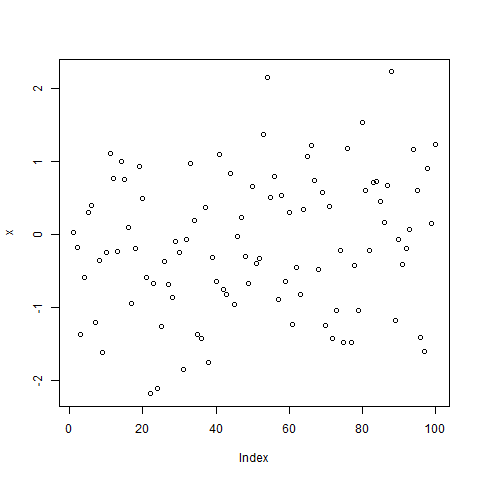
\includegraphics[width=.9\linewidth]{wk4_1.png}

\begin{itemize}
\item but if it is a time series (using \texttt{as.ts} to convert)
\item a different plotting function is dispatched
\end{itemize}

\begin{verbatim}
rm(list=ls())
set.seed(10)
x <- rnorm(100)
x <- as.ts(x)
plot(x)
\end{verbatim}

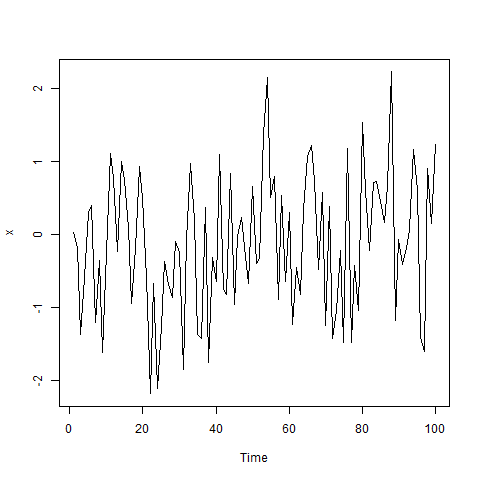
\includegraphics[width=.9\linewidth]{tsFig.png}
\subsubsection{new classes and methods}
\label{sec-4-3-8}

\begin{itemize}
\item Why?
\item You have new data (new to R anyways) without built in ways to manipulate them.
\item new ideas not implimented yet
\item typically write methods for
\item print/show
\item summary
\item plot
\item extend R system via classes and methods
\item write a new class but for existing generic (e.g. \texttt{print})
\item write new generics function and new methods for those generics
\end{itemize}
\subsubsection{S4 methods}
\label{sec-4-3-9}

\begin{itemize}
\item explicity definition for every class
\item use setClass function
\item specify the name of the class (at minimum)
\item data elements (\emph{slots}) which are elements that store data
\item \texttt{setMethod} to define methods
\item \texttt{showClass} gives you information about the class
\end{itemize}
\begin{itemize}

\item Creating new classes/methods
\label{sec-4-3-9-1}%
\begin{itemize}
\item say we want to create a class for \texttt{polygon} explicitly (this is new)
\item usually stored in separate file (sourced into R)
\end{itemize}

\begin{verbatim}
setClass("polygon", representation(x="numeric", y="numeric"))
\end{verbatim}


\begin{itemize}
\item the slots for the class \texttt{polygon} are \texttt{x} and \texttt{y}
\item the slots can be accessed with the \texttt{@} operator
\end{itemize}

A plot method for the \texttt{polygon}


\begin{verbatim}
setMethod("plot", "polygon", function(x,y,...){
    plot(x@x, x@y, type="n", ...)
    xp <- c(x@x, x@x[1])
    yp <- c(x@y, x@y[1])
    lines(xp, yp)

})
\end{verbatim}

\begin{verbatim}
 [1] "plot"
\end{verbatim}

\begin{itemize}
\item notice the \texttt{@} operator to access the slots
\item when run, the setMethod `registers' the method with the system
\item if you close R out - you will have to rededine method
\end{itemize}


\begin{verbatim}
showMethods("plot")
\end{verbatim}

\begin{verbatim}
 Function: plot (package graphics)
 x="ANY", y="ANY"
 x="cenfit", y="ANY"
 x="cenmle-gaussian", y="ANY"
 x="cenmle-lognormal", y="ANY"
 x="cenreg", y="ANY"
 x="polygon", y="ANY"
 x="ros", y="missing"
\end{verbatim}

\begin{itemize}
\item will show that the ploygon method is registered.
\end{itemize}


\begin{verbatim}
p <- new("polygon", x=c(1,2,3,4), y=c(1,2,3,1))
plot(p)
\end{verbatim}

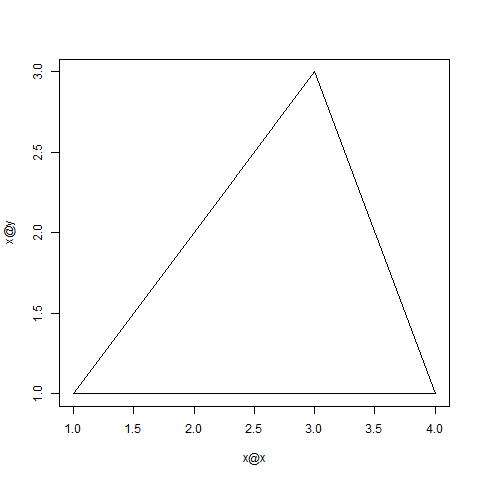
\includegraphics[width=.9\linewidth]{poly.png}

\end{itemize} % ends low level
\subsubsection{places to go to get help}
\label{sec-4-3-10}

\begin{itemize}
\item CRAN (packages that use S4)
\item SparseM, flexm, lme3
\item bioconductor site
\item stats4 (comes with R) has mle methods in S4
\end{itemize}

\end{document}
